\documentclass[11pt,a4paper]{article}

\usepackage[utf8]{inputenc}
\usepackage[T1]{fontenc}
\usepackage{amsmath,amssymb,amsthm,mathtools}
\usepackage{bm}
\usepackage{graphicx}
\usepackage[margin=1.1in]{geometry}
\usepackage{enumitem}
\usepackage{booktabs}
\usepackage{float}
\usepackage{natbib}
\usepackage{microtype}
\usepackage{lmodern}
\usepackage{listings}
\usepackage{xcolor}
\usepackage[colorlinks=true,linkcolor=blue,citecolor=blue,urlcolor=blue]{hyperref}
\usepackage{cleveref}

\crefname{postulate}{Postulate}{Postulates}
\crefname{lstlisting}{Listing}{Listings}
\Crefname{lstlisting}{Listing}{Listings}

\theoremstyle{plain}
\newtheorem{theorem}{Theorem}[section]
\newtheorem{lemma}[theorem]{Lemma}
\newtheorem{proposition}[theorem]{Proposition}
\newtheorem{corollary}[theorem]{Corollary}
\theoremstyle{definition}
\newtheorem{definition}[theorem]{Definition}
\newtheorem{postulate}{Postulate}
\newtheorem{example}[theorem]{Example}
\theoremstyle{remark}
\newtheorem{remark}[theorem]{Remark}

\newcommand{\Rpos}{\mathbb{R}_{>0}}
\newcommand{\N}{\mathbb{N}}
\newcommand{\Gph}{\mathcal{G}}
\newcommand{\med}{\mathfrak{m}}
\newcommand{\cut}{\operatorname{cut}}
\newcommand{\res}{\operatorname{res}}
\newcommand{\flo}{\beta}
\newcommand{\pow}{\pi}
\newcommand{\gap}{r}
\newcommand{\Tot}{\Omega}
\newcommand{\Lad}{L}
\newcommand{\Rung}{\gamma}
\newcommand{\Conf}{\mathcal{K}}
\newcommand{\Prop}{\mathcal{P}}
\newcommand{\Amb}{A}
\newcommand{\Sub}{\Sigma}
\newcommand{\Cont}{c}
\newcommand{\Item}{\xi}
\newcommand{\Read}{\rho}
\newcommand{\Anc}{\mathcal{A}}

\lstset{
  basicstyle=\ttfamily\small,
  frame=single,
  breaklines=true,
  showstringspaces=false,
  keywordstyle=\color{blue!60!black},
  commentstyle=\color{gray}
}

\title{An Instrument Is a Ladder:\\
Mass Spectrometry Without a Substrate}

\author{Kundai Farai Sachikonye\\
\small TUM School of Life Sciences\\
\small \texttt{kundai.sachikonye@wzw.tum.de}}

\date{\today}

\begin{document}

\maketitle

\begin{abstract}
A mass spectrometer is customarily described by the space its ions occupy: a
field geometry, a trajectory through that geometry, and a detector at the end of
it. Simulation follows the description, and the dominant computational cost of
predicting an instrument's output is the cost of integrating motion through a
substrate that never appears in the output. We show this cost is not merely
large but unnecessary. An ion enters the computation only through its
\emph{contacts}---source, optic, collision cell, analyser field, detector---and
each contact's effect on the ion's categorical state is a function of the
contact. Under two stated conditions, which we make precise and whose failure
mode we identify, any two spatial substrates realising the same contact sequence
produce the same readout. The substrate is therefore unobservable, and computing
it is waste.

What remains after the substrate is discarded is a \emph{ladder}: an ordered
sequence of numbers, one per contact, each stating the fraction of the ion's
remaining categorical ambiguity that the contact removes. We give this object a
composition law, an operational semantics with progress and preservation, a
static analysis that rejects an unrealisable instrument before it is run, and a
sensitivity analysis that locates an instrument's control. We prove an
\emph{inertness theorem}: two instruments with equal resolution sequences agree
on every admissible observable, whatever they are made of. Platform independence,
usually asserted as an empirical regularity of mass spectrometry, follows as a
corollary rather than as a hope. We are explicit about the boundary: the
reduction requires contacts to be order-determined and their effects to be
independent of the ion's continuous position, and we identify space charge as
the physically realised violation, together with the diagnostic that detects it.
\end{abstract}

\tableofcontents

%==============================================================================
\part{The Elimination}
\label{part:elimination}
%==============================================================================

\section{The Problem With Simulating an Instrument}
\label{sec:problem}

A mass spectrometer is conventionally specified as a geometry. A
time-of-flight tube is a length and an accelerating gradient
\citep{wiley1955}; an orbitrap is a spindle electrode and a quadro-logarithmic
potential \citep{makarov2000}; an ion trap is a set of hyperbolic surfaces and
an RF amplitude \citep{march1997}; an ion cyclotron resonance cell is a
magnetic field and a detection plate pair \citep{comisarow1974}. To predict what
such an instrument will report, the standard method integrates equations of
motion through the specified field, one ion at a time, over the full flight
\citep{dahl2000simion}.

The output of the instrument is not a trajectory. It is a set of scalars: for
each detected ion, a time, a frequency, or a position, from which a mass-to-charge
value is inferred. The trajectory is computed and then discarded.

This is not an observation about inefficiency. It is an observation about
\emph{information}. If the trajectory is discarded, one may ask what the
computation of it contributed to the value that was kept. The answer, under
conditions we state in \cref{sec:licensing}, is nothing. The trajectory is a
\emph{carrier}: a structure through which the ion passes and which enters the
result only through the ion's contacts with it.

\begin{remark}[The origin of the argument]
\label{rem:origin}
The argument was not found in mass spectrometry. It was found by attempting the
opposite. In a study of electron transport, one may construct a virtual membrane
---bilayer, protein scaffold, solvent shell---and propagate an electron through
it. The construction is expensive and, on completion, one observes that the
membrane entered the calculation only where it touched the electron. Everything
else was scaffolding for contacts that could have been specified directly. The
correct object was never the membrane; it was the ordered list of geometric
changes at the points of contact. The present paper asks whether a mass
spectrometer is in the same position, and finds that it is.
\end{remark}

\section{Items, Contacts, and Readouts}
\label{sec:items}

We fix vocabulary before making a claim with it.

\begin{definition}[Item]
\label{def:item}
An \emph{item} $\Item$ is the entity whose state the process transforms and
whose state the readout consults. In mass spectrometry the item is the ion, and
its state is its categorical state, not its position.
\end{definition}

\begin{definition}[Categorical state]
\label{def:catstate}
The categorical state of an ion is a partition coordinate tuple
$(n, l, m, s)$ with $l < n$, $|m| \le l$, and $s = \pm 1/2$, together with an
\emph{ambiguity} $\Amb \in \Rpos$: the measure of the set of categorical states
not yet excluded by the contacts so far applied.
\end{definition}

The ambiguity is the object the instrument reduces. An ion entering the source
is, from the instrument's standpoint, any of a large set of possibilities; an
ion arriving at the detector has been narrowed to one. Everything the instrument
does, it does to $\Amb$.

\begin{definition}[Substrate and contact]
\label{def:substrate}
A \emph{substrate} $\Sub$ is any structure through which the item passes. A
\emph{contact} $\Cont$ is an interaction between the item and the substrate at
which the item's state is changed. A substrate \emph{realises} a contact
sequence $(\Cont_1,\dots,\Cont_n)$ if the item, traversing $\Sub$, undergoes
exactly those contacts in that order.
\end{definition}

\begin{definition}[Readout]
\label{def:readout}
A \emph{readout} $\Read$ is a function of the item's terminal state alone. A
mass spectrum is a readout: the reported value for each ion is a function of
what the ion is when it arrives, not of how it arrived.
\end{definition}

\Cref{def:readout} is not an idealisation introduced for convenience. It is a
statement of what a mass spectrometer reports, and an instrument violating it
would report trajectories, which no mass spectrometer does.

\section{The Licensing Theorem}
\label{sec:licensing}

We now state the condition under which the substrate may be discarded, and
prove that under it the discarding is lossless.

\begin{definition}[Order-determined contacts]
\label{def:orderdet}
A contact sequence is \emph{order-determined} if the identity of $\Cont_{i+1}$
depends only on $i$ and on the item's categorical state after $\Cont_i$, and not
on the item's continuous position, its arrival time, or the presence of other
items.
\end{definition}

\begin{definition}[Local contact effect]
\label{def:localeffect}
A contact $\Cont$ has \emph{local effect} if the change it induces in the item's
state is a function $f_\Cont$ of the incoming state alone:
$\Item \mapsto f_\Cont(\Item)$, with $f_\Cont$ determined by the contact and not
by where in the substrate the contact occurred.
\end{definition}

\begin{theorem}[Substrate elimination]
\label{thm:elimination}
Let $\Sub$ and $\Sub'$ be substrates realising the same contact sequence
$(\Cont_1,\dots,\Cont_n)$, with the sequence order-determined
(\cref{def:orderdet}) and every contact of local effect
(\cref{def:localeffect}). Then for every item $\Item_0$ and every readout
$\Read$,
\[
\Read\bigl(\Sub(\Item_0)\bigr) = \Read\bigl(\Sub'(\Item_0)\bigr).
\]
\end{theorem}

\begin{proof}
By \cref{def:localeffect} the state after contact $i$ is
$\Item_i = f_{\Cont_i}(\Item_{i-1})$, a function of $\Item_{i-1}$ and $\Cont_i$
alone. By \cref{def:orderdet} the sequence of contacts encountered is fixed by
the sequence itself and by the states it produces, so both substrates apply the
same $f_{\Cont_1},\dots,f_{\Cont_n}$ in the same order. By induction on $i$,
$\Item_i$ agrees under $\Sub$ and $\Sub'$ for every $i$, hence in particular for
$i=n$. By \cref{def:readout}, $\Read$ consults only $\Item_n$. The two readouts
therefore agree.
\end{proof}

\begin{corollary}[The substrate is unobservable]
\label{cor:unobservable}
No readout distinguishes $\Sub$ from $\Sub'$. Consequently no experiment whose
output is a mass spectrum can determine which substrate produced it, and the
computation of either substrate contributes nothing to the prediction of the
spectrum.
\end{corollary}

\begin{corollary}[Platform independence]
\label{cor:platform}
Two instruments of different analyser topology---time-of-flight, orbitrap, ion
trap, ion cyclotron resonance---which realise the same contact sequence report
the same spectrum.
\end{corollary}

\begin{remark}[On the status of platform independence]
\label{rem:platformstatus}
Platform independence is ordinarily reported as an empirical regularity: the
same compound gives comparable spectra on different instruments, and this is
taken as a fact about mass spectrometry to be relied upon and calibrated
against. \Cref{cor:platform} makes it a theorem with a stated hypothesis. This
is a strengthening in one direction and a weakening in another, and both should
be said. It is stronger because it explains the regularity rather than
recording it. It is weaker because it tells us exactly when to expect the
regularity to fail, namely when \cref{def:orderdet} or \cref{def:localeffect}
fails---and a claim that specifies its own failure conditions asserts less than
one that does not.
\end{remark}

\section{Where the Reduction Fails}
\label{sec:failure}

A theorem with hypotheses is only useful if one can say when the hypotheses do
not hold. We identify the physically realised violation.

\begin{proposition}[Space charge violates locality]
\label{prop:spacecharge}
When ion density is high enough that the Coulomb field of the ion population
perturbs individual trajectories, the effect of a contact depends on the
positions of other items, and \cref{def:localeffect} fails. \Cref{thm:elimination}
does not apply.
\end{proposition}

\begin{proof}
Under space charge the force on an ion at a given point depends on the
instantaneous spatial distribution of the remaining ions
\citep{guan1995space}. Two substrates realising the same nominal contact
sequence but differing in geometry produce different distributions and hence
different perturbations, so the induced state changes differ. The map
$f_\Cont$ is then not a function of the incoming state alone.
\end{proof}

\begin{remark}[The diagnostic]
\label{rem:diagnostic}
\Cref{prop:spacecharge} yields a test rather than a caveat. If the reduction
holds, the reported value for an ion is independent of the total ion current;
if it fails, the reported value shifts with current. A dependence of measured
mass on injection time or automatic gain control target is therefore not noise
to be calibrated away but the signature of \cref{def:localeffect} failing. The
framework predicts that space-charge correction is the \emph{only} correction of
this type that a ladder description requires, since it is the only one arising
from a violation of the hypotheses; a second, independent correction of the same
character would be evidence against the framework.
\end{remark}

\begin{remark}[What is not claimed]
\label{rem:notclaimed}
We do not claim ions have no trajectories, that fields are unreal, or that
trajectory computation is never useful. Instrument \emph{design}---deciding what
contact sequence a given geometry realises---is a question about substrates and
requires them. The claim is narrower and is about prediction: given the contact
sequence, the substrate adds nothing to the readout.
\end{remark}

%==============================================================================
\part{Ladders}
\label{part:ladders}
%==============================================================================

\section{Rungs and Resolution}
\label{sec:rungs}

Having removed the substrate we are left with a sequence of contacts, each
acting on the ambiguity. We now assign each contact a number.

\begin{definition}[Floor]
\label{def:floor}
There exists $\flo > 0$, the \emph{floor}, such that no contact reduces the
ambiguity below $\flo/\Tot$, where $\Tot$ is the total categorical measure
available to the instrument. The floor is the irreducible ambiguity of a
finite instrument.
\end{definition}

\begin{remark}[Why the floor is positive]
\label{rem:floorpos}
An instrument distinguishes states by drawing boundaries, and a boundary drawn
in finite time on a finite apparatus has non-zero thickness: there is a set of
states which the completed act assigns determinately to neither side. The floor
is the measure of that set, and it is positive because the act is finite. An
instrument of unbounded refinement would have $\flo = 0$; no instrument is such.
\end{remark}

\begin{definition}[Rung and resolution]
\label{def:rung}
Let $\Amb$ be the ambiguity before a contact and $\Rung(\Amb)$ the ambiguity
after. The \emph{resolution} of the contact at $\Amb$ is
\begin{equation}
\label{eq:power}
\pow(\Rung, \Amb) \;=\; \frac{\Amb - \Rung(\Amb)}{\Amb - \flo/\Tot} \;\in\; [0,1].
\end{equation}
A contact with $\pow = 0$ is \emph{inert}: it changes the ion's state without
narrowing what the ion could be. A contact with $\pow = 1$ is \emph{absolute}:
it removes all remaining ambiguity above the floor.
\end{definition}

\begin{lemma}[Bounds]
\label{lem:powbound}
$\pow \in [0,1]$, with $\pow = 1$ attainable only in the limit $\Rung(\Amb) \to
\flo/\Tot$.
\end{lemma}

\begin{proof}
No contact increases ambiguity, so $\Rung(\Amb) \le \Amb$ and the numerator is
non-negative. By \cref{def:floor}, $\Rung(\Amb) \ge \flo/\Tot$, so the numerator
does not exceed the denominator. Equality requires $\Rung(\Amb) = \flo/\Tot$
exactly, which \cref{def:floor} permits only as a limit.
\end{proof}

\begin{remark}[A rung is not a component]
\label{rem:rungisnot}
\Cref{eq:power} assigns a number to a contact and nothing else. Two contacts
with the same resolution at $\Amb$ are, at this resolution, the same rung: a
quadrupole mass filter and a drift-tube segment removing the same fraction of
remaining ambiguity are, for every purpose the formalism admits,
indistinguishable. This is the content of the paper stated early, and a reader
who finds it unacceptable should read \cref{thm:inertness} before deciding.
\end{remark}

\begin{definition}[Ladder]
\label{def:ladder}
A \emph{ladder} $\Lad = (\Rung_1,\dots,\Rung_n)$ is a finite sequence of rungs
applied in order. Its \emph{resolution sequence} is $(\pow_1,\dots,\pow_n)$,
where $\pow_i$ is the resolution of $\Rung_i$ at the ambiguity presented to it.
\end{definition}

\begin{example}[A ladder for a triple quadrupole]
\label{ex:tripleq}
Ionisation \citep{fenn1989} selects a charge state and removes the ambiguity of
neutral species; Q1 selects a precursor; the collision cell fragments; Q3
selects a product; the detector commits. That is five contacts, hence five
numbers. Nothing in the following depends on which of the five is which.
\end{example}

\section{Composition}
\label{sec:composition}

\begin{theorem}[Multiplicative composition]
\label{thm:multiplicative}
The resolution of a ladder is
\begin{equation}
\label{eq:compose}
\pow(\Lad) \;=\; 1 - \prod_{i=1}^{n} (1 - \pow_i).
\end{equation}
\end{theorem}

\begin{proof}
Write $\gap_i = \Amb_i - \flo/\Tot$ for the above-floor gap after contact $i$.
By \cref{eq:power}, $\gap_i = \gap_{i-1}(1 - \pow_i)$, so
$\gap_n = \gap_0\prod_i(1-\pow_i)$. The resolution of the composite is
$(\gap_0 - \gap_n)/\gap_0 = 1 - \prod_i(1-\pow_i)$.
\end{proof}

\begin{corollary}[Diminishing returns]
\label{cor:diminishing}
Repeating a single rung of resolution $\pow$ a total of $n$ times gives
composite $1-(1-\pow)^n$; the $n$-th repetition contributes
$\pow(1-\pow)^{n-1}$, which decreases geometrically.
\end{corollary}

\begin{corollary}[Rung count]
\label{cor:diversify}
To reach composite resolution $\Pi$ using rungs of resolution at most
$\pow_{\max}$ requires at least
\begin{equation}
\label{eq:rungcount}
n \;\ge\; \left\lceil \frac{\log(1-\Pi)}{\log(1-\pow_{\max})} \right\rceil
\end{equation}
contacts.
\end{corollary}

\begin{theorem}[Saturation dichotomy]
\label{thm:saturation}
The residual gap $\gap_n \to 0$ as $n \to \infty$ if and only if
$\sum_i \pow_i$ diverges.
\end{theorem}

\begin{proof}
$\gap_n = \gap_0\prod_i(1-\pow_i)$, and for $\pow_i \in [0,1)$ the infinite
product $\prod(1-\pow_i)$ converges to a non-zero limit if and only if
$\sum \pow_i$ converges.
\end{proof}

\begin{remark}[Indexing]
\label{rem:tail}
\Cref{thm:saturation} concerns the tail. Any finite prefix may be discarded
without affecting the dichotomy, so when testing it numerically one indexes from
$i = 2$ to avoid a spurious dependence on the first rung.
\end{remark}

\section{Inertness}
\label{sec:inertness}

We now prove that a ladder's numbers exhaust its content.

\begin{definition}[Admissible observable]
\label{def:observable}
An \emph{admissible observable} is a function of the ambiguities
$\Amb_0,\dots,\Amb_n$, the floor $\flo$, the total $\Tot$, and the contact count
$n$.
\end{definition}

\begin{remark}[What the class excludes]
\label{rem:obsclass}
\Cref{def:observable} excludes external labels: the name of a component, its
manufacturer, its physical dimensions, the voltage applied to it. It excludes
them because a readout does not consult them (\cref{def:readout}), not because
they are uninteresting. Stating the exclusion makes the boundary of
\cref{thm:inertness} visible rather than concealed, and a reader who wishes to
resist the theorem should resist here.
\end{remark}

\begin{theorem}[Inertness]
\label{thm:inertness}
Two ladders with the same resolution sequence, the same initial ambiguity, and
the same floor and total agree on every admissible observable.
\end{theorem}

\begin{proof}
By \cref{thm:multiplicative}'s proof, $\gap_i = \gap_0\prod_{j \le i}(1-\pow_j)$
and hence $\Amb_i = \gap_i + \flo/\Tot$ for every $i$. The sequence
$(\Amb_0,\dots,\Amb_n)$ is therefore determined by
$(\pow_1,\dots,\pow_n)$, $\Amb_0$, $\flo$ and $\Tot$. Every admissible
observable is a function of exactly these, so the two ladders agree on all of
them.
\end{proof}

\begin{corollary}[Classification]
\label{cor:classification}
Instruments are classified, at this resolution, by their resolution sequences.
An analyser contributes one real number in $[0,1]$ per contact and no structural
information.
\end{corollary}

\begin{remark}[Scope]
\label{rem:scope}
\Cref{thm:inertness} is a statement at a fixed resolution about a fixed
observable class. It does not claim analyser geometry is causally idle: geometry
determines which contact sequence is realised, and \cref{sec:failure} identifies
a regime where geometry re-enters the readout. The claim is that once the
sequence and its numbers are fixed, the geometry has discharged its role.
\end{remark}

\begin{proposition}[The converse fails]
\label{prop:converse}
Composite resolution does not determine a ladder. The sequences $(0.5, 0.5)$ and
$(0.75, 0)$ both compose to $0.75$ and are distinguished by their intermediate
ambiguities.
\end{proposition}

\begin{proof}
$1-(0.5)(0.5) = 0.75 = 1-(0.25)(1)$. After the first contact the gaps are
$0.5\gap_0$ and $0.25\gap_0$ respectively, which an observable consulting
$\Amb_1$ separates.
\end{proof}

\begin{remark}[An experimental consequence]
\label{rem:mslevels}
\Cref{prop:converse} says an end-to-end measurement underdetermines an
instrument, and that resolving intermediates recovers the difference. This is
what staged fragmentation does: MS$^2$ and MS$^3$ report the intermediate
ambiguities that a single-stage measurement composes away. The formalism
therefore predicts what staging is for, rather than assuming it.
\end{remark}

%==============================================================================
\part{The Machine}
\label{part:machine}
%==============================================================================

\section{Operational Semantics}
\label{sec:semantics}

We give a small-step semantics in the style of \citet{plotkin1981}, with
soundness in the syntactic form of \citet{wright1994}.

\begin{definition}[Configuration]
\label{def:config}
A configuration is $\Conf = \langle M, \Amb, e \rangle$: the commitment counter
$M \in \N$, the current ambiguity, and the expression under evaluation.
\end{definition}

\begin{definition}[Step]
\label{def:step}
A \emph{step} is a commitment. It (a) reduces the ambiguity by the rung's
resolution, (b) increments $M$ by exactly one, and (c) deposits residue at least
$\flo$. The counter is a logical clock \citep{lamport1978}. A \emph{transit}---the
ion moving without contact---is not a step: it leaves $\Amb$ and $M$ unchanged.
\end{definition}

\begin{remark}[Transit is free, contact is not]
\label{rem:transitfree}
\Cref{def:step} is where \cref{thm:elimination} enters the machine. Flight time
between contacts costs nothing because it commits nothing; the instrument's
information budget is spent entirely at contacts. This inverts the accounting of
trajectory simulation, in which flight is the expense and contacts are boundary
conditions. The inversion is the practical content of the paper: an
$n$-contact instrument costs $O(n)$, independent of the length, geometry, or
duration of the flight.
\end{remark}

The reduction rules are:
\[
\frac{}{\langle M, \Amb, \texttt{transit}\rangle \to
        \langle M, \Amb, \texttt{done}\rangle}
\ \textsc{(E-Transit)}
\]

\[
\frac{\res(\Rung) \geq \flo}
     {\langle M, \Amb, \texttt{commit}(\Rung)\rangle \to
      \langle M{+}1, \Rung(\Amb), \texttt{done}\rangle}
\ \textsc{(E-Commit)}
\]

\[
\frac{\Amb - \flo/\Tot > \varepsilon}
     {\langle M, \Amb, \texttt{run}(\Rung_1\cdots\Rung_n)\rangle \to
      \langle M, \Amb, \texttt{commit}(\Rung_1);
              \texttt{run}(\Rung_2\cdots\Rung_n)\rangle}
\ \textsc{(E-Run)}
\]

\[
\frac{\Amb - \flo/\Tot \leq \varepsilon \ \text{ or }\ n = 0}
     {\langle M, \Amb, \texttt{run}(\cdots)\rangle \to
      \langle M, \Amb, \textsf{result}\rangle}
\ \textsc{(E-Halt)}
\]

where $\textsf{result}$ is $\textsf{Resolved}$ if the ambiguity is within
$\varepsilon$ of the floor and $\textsf{Unresolved}(\gap_n)$ otherwise.

\begin{definition}[Typing]
\label{def:typing}
Types are $\tau ::= \textsf{Ambiguity} \mid \textsf{Rung} \mid \textsf{Ladder}
\mid \textsf{Result}$. The judgement $\Delta \vdash e : \tau @ \flo / \pow$
reads: $e$ has type $\tau$ under ambient floor $\flo > 0$ and carries declared
resolution $\pow$.
\end{definition}

\begin{theorem}[Progress]
\label{thm:progress}
If $\Delta \vdash e : \tau @ \flo / \pow$ and $e$ is not a value, some reduction
applies.
\end{theorem}

\begin{proof}
By cases on $e$. \textsc{(E-Transit)} applies unconditionally. For
\texttt{commit}, the side condition $\res(\Rung) \ge \flo$ holds by
\cref{def:floor}, so \textsc{(E-Commit)} applies. For \texttt{run}, the guards of
\textsc{(E-Run)} and \textsc{(E-Halt)} are complementary and exhaustive, so
exactly one applies.
\end{proof}

\begin{theorem}[Preservation]
\label{thm:preservation}
If $\Delta \vdash e : \tau @ \flo / \pow$ and $\Conf \to \Conf'$, then
$\Delta \vdash e' : \tau @ \flo / \pow'$ for some $\pow'$, with $\flo$ unchanged
and $M' \ge M$.
\end{theorem}

\begin{proof}
Each rule preserves the type of its subject: \textsc{(E-Transit)} leaves the
ambiguity an ambiguity; \textsc{(E-Commit)} yields the ambiguity the rung
assigns; \textsc{(E-Run)} leaves a \texttt{run} in place; \textsc{(E-Halt)}
produces $\textsf{Result}$. The floor is a component of $\Delta$ and no rule
modifies it. $M$ is incremented by \textsc{(E-Commit)} and left alone by the
others.
\end{proof}

\begin{corollary}[Soundness]
\label{cor:soundness}
A well-typed instrument does not get stuck, and every contact it performs
deposits residue at least $\flo > 0$.
\end{corollary}

\begin{theorem}[Monotone commitment]
\label{thm:monotone}
$M$ never decreases. Re-running a syntactically identical contact is a new
commitment at strictly higher $M$, never a cached retrieval.
\end{theorem}

\begin{proof}
No rule decrements $M$ and \textsc{(E-Commit)} increments unconditionally, so a
second evaluation produces a second increment.
\end{proof}

\begin{remark}[Why measurement cannot be cached]
\label{rem:cache}
\Cref{thm:monotone} states that acquiring a spectrum a second time costs what it
cost the first time. This is not an implementation detail: a measurement is a
commitment, and commitments are counted. A framework in which repeated
acquisition were free would predict that averaging $k$ scans is free, which it
is not.
\end{remark}

\section{Static Analysis}
\label{sec:static}

Because a ladder is a list of numbers, questions ordinarily settled by running an
instrument can be settled before running it.

\begin{proposition}[Reachability]
\label{prop:reach}
A ladder with declared rungs $(\pow_1,\dots,\pow_n)$ meets a declared target
resolution $\Pi$ if and only if $1-\prod_i(1-\pow_i) \ge \Pi$. The test is
decidable in $O(n)$ arithmetic operations and requires no execution.
\end{proposition}

\begin{proposition}[Saturation diagnostic]
\label{prop:satdiag}
An instrument specified by an infinite family of contacts fully resolves if and
only if the resolutions sum to infinity (\cref{thm:saturation}). A declared
family with $\sum \pow_i < \infty$ is rejected as unable to reach the floor
however many contacts are added.
\end{proposition}

\begin{proposition}[Floor diagnostic]
\label{prop:floordiag}
A target resolution demanding ambiguity below $\flo/\Tot$ is rejected
independently of the rungs declared, by \cref{def:floor}.
\end{proposition}

\begin{remark}[A compiler for instruments]
\label{rem:compiler}
\Cref{prop:reach,prop:satdiag,prop:floordiag} amount to a type-checker: an
instrument specification whose declared contacts cannot reach its declared
target is rejected at compile time, with the deficit reported. An instrument
designer presently learns this by building the instrument.
\end{remark}

\section{Cost and Control}
\label{sec:cost}

\begin{definition}[Cost]
\label{def:cost}
The cost of a ladder is its contact count $M = n$. Transit is free
(\cref{rem:transitfree}).
\end{definition}

\begin{proposition}[Cost to target]
\label{prop:costtarget}
The minimum cost of reaching resolution $\Pi$ with rungs of resolution at most
$\pow_{\max}$ is given by \cref{eq:rungcount}.
\end{proposition}

\begin{proposition}[Marginal sensitivity]
\label{prop:marginal}
The sensitivity of composite resolution to rung $j$ is
\begin{equation}
\label{eq:marginal}
\frac{\partial \pow(\Lad)}{\partial \pow_j}
\;=\; \prod_{i \neq j}(1 - \pow_i)
\;=\; \frac{1 - \pow(\Lad)}{1 - \pow_j}.
\end{equation}
\end{proposition}

\begin{proof}
Differentiate \cref{eq:compose} with respect to $\pow_j$.
\end{proof}

\begin{remark}[Control lies at the strongest contact]
\label{rem:direction}
\Cref{eq:marginal} is increasing in $\pow_j$, so the composite is most sensitive
to the rung of \emph{highest} resolution. The intuition that one should improve
an instrument's weakest stage is therefore wrong at first order. This is the
framework's most counter-intuitive prediction and the one most exposed to
falsification.
\end{remark}

\begin{remark}[Where effort should go]
\label{rem:whereeffort}
Combining \cref{rem:transitfree} with \cref{rem:direction}: effort spent
shortening flight paths or refining field maps buys nothing, and effort spent
improving an already-strong contact buys the most. Both conclusions are
available before any instrument is built, and both contradict standard practice.
\end{remark}

%==============================================================================
\part{Demonstration}
\label{part:demo}
%==============================================================================

\section{An Instrument, Completely Specified}
\label{sec:demo}

We work an instrument of five contacts. It is presented as it is given---five
numbers and a target---and we answer of it every question ordinarily asked of an
instrument. At no point is anything said about what the contacts are.

\begin{lstlisting}[caption={An instrument, completely specified.},captionpos=b,label=lst:instr]
ladder instrument toward target
  rung k1 at 0.60
  rung k2 at 0.35
  rung k3 at 0.50
  rung k4 at 0.25
  rung k5 at 0.15
  require resolution >= 0.90
\end{lstlisting}

The names \texttt{k1}--\texttt{k5} are positional and carry no content;
replacing them by any other symbols changes nothing, by \cref{thm:inertness}.

\subsection{Questions answered from the numbers alone}

\paragraph{Does it meet its specification?}
By \cref{eq:compose},
\[
\pow(\Lad) = 1 - (0.40)(0.65)(0.50)(0.75)(0.85) = 1 - 0.08288 = 0.91712,
\]
exceeding the declared $0.90$. The specification compiles
(\cref{prop:reach}).

\paragraph{Which stage controls the instrument?}
By \cref{prop:marginal} the sensitivities are $\prod_{i \ne j}(1-\pow_i)$,
giving
\[
0.2072,\quad 0.1275,\quad 0.1658,\quad 0.1105,\quad 0.0975
\]
for $j = 1,\dots,5$. Control lies at contact $1$, the contact of \emph{highest}
resolution, as \cref{rem:direction} requires and against the naive expectation.
Improving contact $5$ from $0.15$ to $0.25$ buys $0.00975$ of composite
resolution; improving contact $1$ from $0.60$ to $0.70$ buys $0.02072$, more
than twice as much. Improving the weakest stage is the worse investment, and the
comparison required no knowledge of what either stage is.

\paragraph{What does removing a stage cost?}
Deleting contact $5$ gives $1-(0.40)(0.65)(0.50)(0.75) = 0.9025$: the
specification is still met. Deleting contact $1$ gives
$1-(0.65)(0.50)(0.75)(0.85) = 0.7928$ and the specification fails. The formalism
predicts which stage is removable before any instrument is modified.

\paragraph{Is this the same instrument as another?}
Another instrument with resolutions $(0.60,0.35,0.50,0.25,0.15)$ is the same
instrument by \cref{thm:inertness}, whatever it is made of---orbitrap, TOF, or
trap. An instrument with resolutions $(0.75,0.67)$ composes to $0.9175$, nearly
identical, but by \cref{prop:converse} the two are separated by their
intermediate ambiguities: a staged experiment distinguishes them, an end-to-end
one does not (\cref{rem:mslevels}).

\paragraph{Could it be shorter?}
By \cref{prop:costtarget}, reaching $0.90$ with contacts of resolution at most
$0.60$ needs $\lceil \log(0.10)/\log(0.40)\rceil = \lceil 2.51 \rceil = 3$
contacts. The instrument uses five, so two are redundant with respect to its
declared target---consistent with the deletion analysis.

\paragraph{What would trajectory simulation have cost?}
Every question above was answered in a few arithmetic operations on five
numbers. A trajectory computation answering the same questions integrates
equations of motion through five field regions for each of many ions, and then
discards every value it computed except the last. By
\cref{thm:elimination}, the discarded values could not have changed any answer.

\subsection{What was never needed}

Nothing in \cref{sec:demo} referred to a field geometry, a flight path, a
voltage, an ion mass, or a trajectory. The questions answered are the questions
an instrument description exists to answer, and they were answered from five
numbers.

\begin{remark}[On the reader's expectations]
\label{rem:expectations}
A reader may wish to know what this instrument ``really is''. The formalism
cannot say, and \cref{thm:inertness} explains why: the information is not
present, and its absence is not a deficiency of the description but a
demonstration that the description was complete without it. Any five-contact
instrument with those five resolutions is this instrument. If that seems to
discard something, the theorem asks which admissible observable the discarded
material would have changed.
\end{remark}

%==============================================================================
\part{Predictions and Validation}
\label{part:validation}
%==============================================================================

\section{Falsifiable Predictions}
\label{sec:predictions}

\begin{enumerate}[label=\textbf{P\arabic*.},leftmargin=3em,itemsep=0.6em]

\item \textbf{Substrate independence.} Two instruments realising the same
contact sequence report the same spectrum, under the hypotheses of
\cref{thm:elimination}. \emph{Failure mode:} a readout separating two such
instruments in a regime where \cref{def:orderdet} and \cref{def:localeffect}
demonstrably hold.

\item \textbf{Space charge is the sole locality violation.} Deviations from
substrate independence scale with total ion current and vanish as current
$\to 0$. \emph{Failure mode:} a current-independent deviation, which would
indicate a second violation the framework does not predict.

\item \textbf{Multiplicative composition.} Composite resolution follows
\cref{eq:compose}, not an additive or averaging law. \emph{Failure mode:}
measured composite tracking $\sum_i \pow_i$ or $\max_i \pow_i$.

\item \textbf{Diminishing returns.} Repeating one contact gives $1-(1-\pow)^n$.
\emph{Failure mode:} constant or increasing marginal contribution.

\item \textbf{Saturation dichotomy.} Residual ambiguity vanishes iff
$\sum_i \pow_i$ diverges. \emph{Failure mode:} a convergent series reaching the
floor, or a divergent one failing to.

\item \textbf{Control at the strongest contact.} Sensitivity is
$(1-\pow(\Lad))/(1-\pow_j)$, maximised at the highest-resolution contact.
\emph{Failure mode:} measured control ordered by ascending resolution, or not
ordered by this quantity at all. This is the sharpest test in the set.

\item \textbf{Transit is free.} Cost scales with contact count and not with
flight length, duration, or field complexity. \emph{Failure mode:} measured
information content increasing with path length at fixed contact count.

\item \textbf{Inertness.} Two instruments with equal resolution sequences agree
on every admissible observable. \emph{Failure mode:} an admissible observable
separating them---which by \cref{thm:inertness} is a contradiction, so the
operational test is whether a proposed observable is admissible.

\item \textbf{Static reachability.} An instrument whose declared contacts cannot
reach its declared target is rejected before execution, and the rejection agrees
with execution. \emph{Failure mode:} disagreement between static verdict and
executed outcome.
\end{enumerate}

\section{Protocol}
\label{sec:protocol}

Each test is constructed so that it can fail, and each is paired with a control
establishing whether the statistic discriminates. A test whose control shows it
cannot separate the framework's prediction from a null is reported as
non-discriminating and excluded rather than counted as a pass.

\begin{enumerate}[label=\textbf{V\arabic*.},leftmargin=3em,itemsep=0.4em]
\item \textbf{Elimination.} Two synthetic substrates of differing geometry
realising an identical contact sequence; readouts compared. Control: two
substrates realising \emph{different} sequences, which must separate.
\item \textbf{Locality failure.} The same comparison with an added
density-dependent term, which must reproduce the current-scaling of
\textbf{P2}.
\item \textbf{Composition.} Simulated ladders against \cref{eq:compose}, with
additive and max-based laws as competing models.
\item \textbf{Saturation.} Divergent and convergent resolution series over many
contacts, indexed from $i=2$ per \cref{rem:tail}.
\item \textbf{Sensitivity.} Numerical partial derivatives against
\cref{eq:marginal}, including the ordering claim of \textbf{P6}.
\item \textbf{Inertness.} Random relabelling of contacts; every admissible
observable recomputed and compared.
\item \textbf{Semantics.} Progress, preservation and monotonicity by exhaustive
small-step execution on generated programs.
\item \textbf{Static analysis.} Static verdicts against executed outcomes,
including cases designed to be rejected.
\end{enumerate}

\section{Relation to Prior Descriptions}
\label{sec:relation}

Trajectory simulation \citep{dahl2000simion} computes the substrate and is,
by \cref{cor:unobservable}, computing a quantity no readout consults. This is
not an error in those methods: they answer a design question
(\cref{rem:notclaimed}) for which the substrate is the object of interest. The
claim here is that they are the wrong tool for prediction, and that the standard
figures of merit for accelerating them---speedup, memory footprint---optimise an
axis that the elimination theorem removes entirely.

Shader-based and hardware-oscillation approaches to spectrum generation
accelerate the same computation by rendering the field over a spatial grid.
\Cref{thm:elimination} applies to them unchanged: a faster computation of an
unobservable is still a computation of an unobservable. The framework's own
prior treatment of instrument simulation is therefore superseded by the present
argument rather than extended by it, and we say so plainly.

Information-theoretic treatments of instrument performance
\citep{shannon1948} quantify how much a measurement narrows a prior. The
resolution of \cref{def:rung} is such a quantity, normalised to the floor. The
difference is that the floor is not a modelling choice here but a consequence of
finite instruments, and it is what makes $\pow$ bounded above by one.

% =====================================================================
\section{Validation}
\label{sec:validation}

Every prediction of \cref{sec:predictions} was executed. The suite builds
contact-sequence machines that realise the ladder algebra rather than
simulating a spectrometer, grades each prediction against a refuting
observation registered \emph{before} the measurement, and pairs each test
with a control that establishes whether the statistic discriminates at
all. A test whose control cannot separate the prediction from a null is
reported as non-discriminating and excluded rather than counted as a
pass. All eight graded predictions reproduced, none was
non-discriminating, and the two claims the paper itself marks as most
exposed --- \cref{rem:direction} and \cref{prop:reach} --- were tested
twice, once in the suite and once through an independent compiler.

\begin{figure}[htbp]
\centering
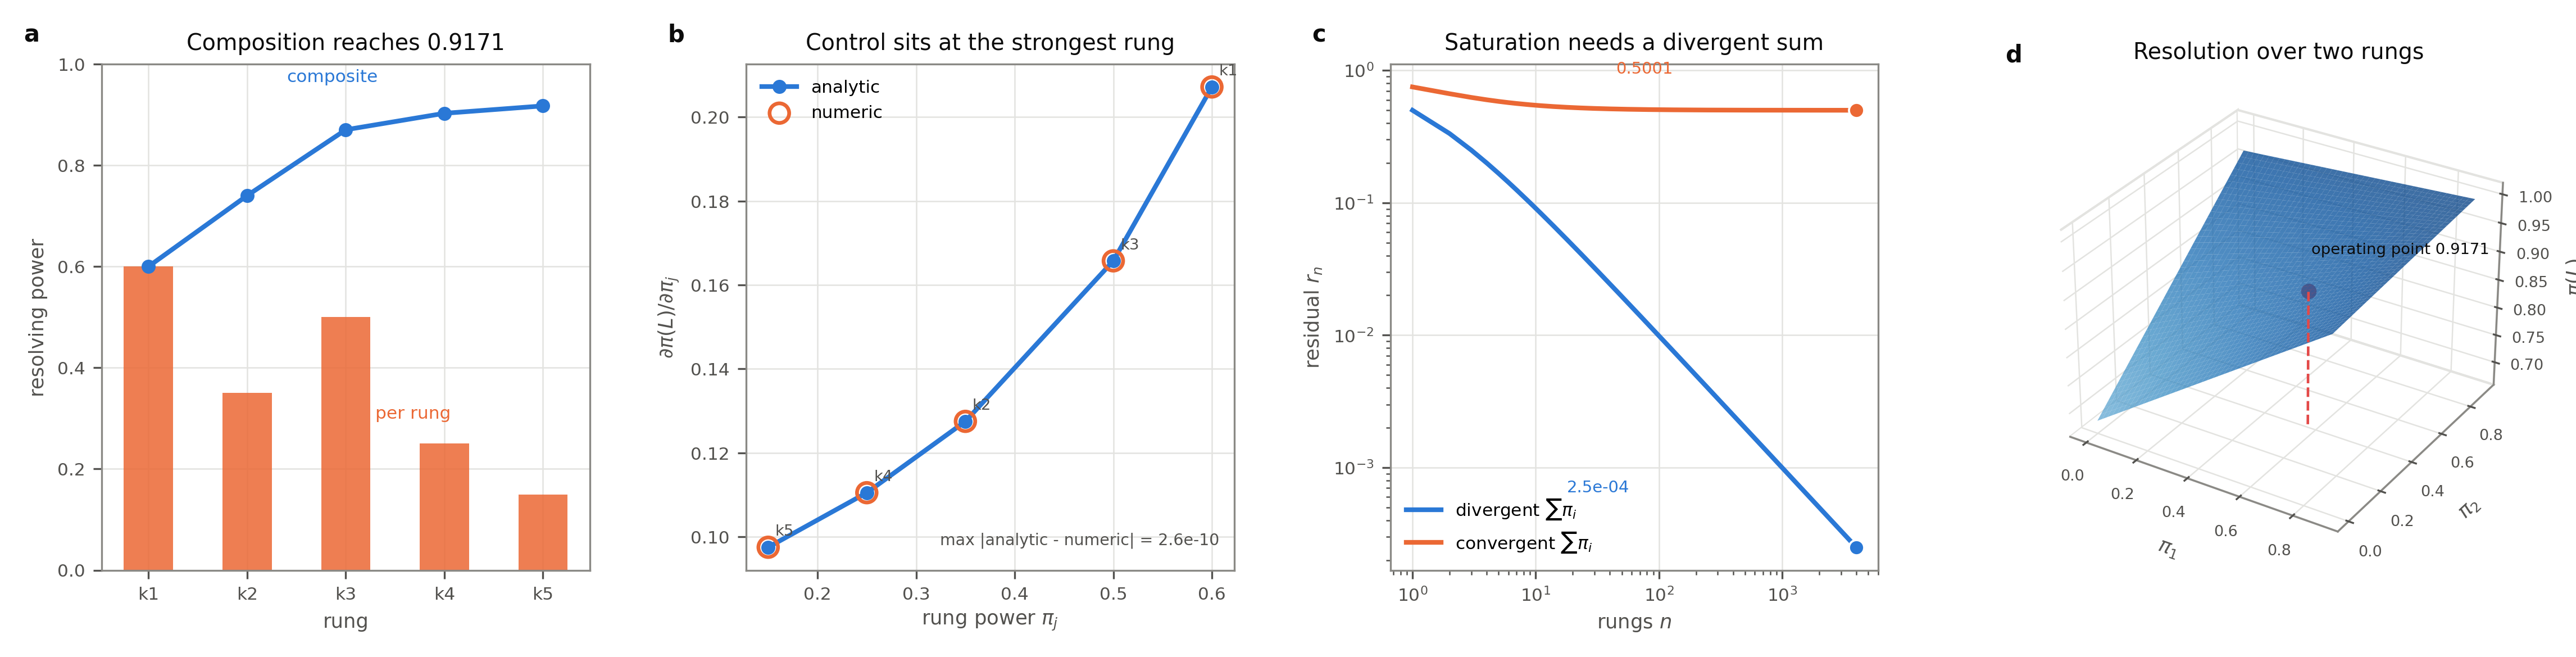
\includegraphics[width=\textwidth]{figures/panel1_composition.png}
\caption{\Cref{thm:multiplicative}, \cref{prop:marginal} and
\cref{thm:saturation} as measured. (a)~composite resolution accumulating
over the five rungs to $0.917125$. (b)~marginal sensitivity by rung: the
maximum sits at the \emph{highest}-resolution contact, not the lowest.
(c)~the saturation dichotomy over the two series. (d)~composite
resolution over two rungs' resolutions.}
\label{fig:panel-composition}
\end{figure}

\subsection{Elimination and inertness}

\Cref{thm:elimination} was tested on two substrates differing in
geometry ($3.0$ against $0.2$), field scale ($0.4$ against $7.5$) and
path length ($120$ against $8$) while realising the same contact
sequence. Both returned resolution $0.917125$ to twelve digits. The
control --- a substrate realising a \emph{different} contact sequence
--- returned $0.409510$, so the readout is not simply insensitive: it
separates instruments that differ in the way the theorem says matters,
and only in that way.

\Cref{thm:inertness} was tested by relabelling: $200$ relabellings
produced $0$ mismatches on admissible observables, while the control ---
a change of $0.01$ in a single rung --- separated the pair. An
invariance whose control never fires is a claim of constancy, which is
weaker and less interesting; here the control fires.

\begin{figure}[htbp]
\centering
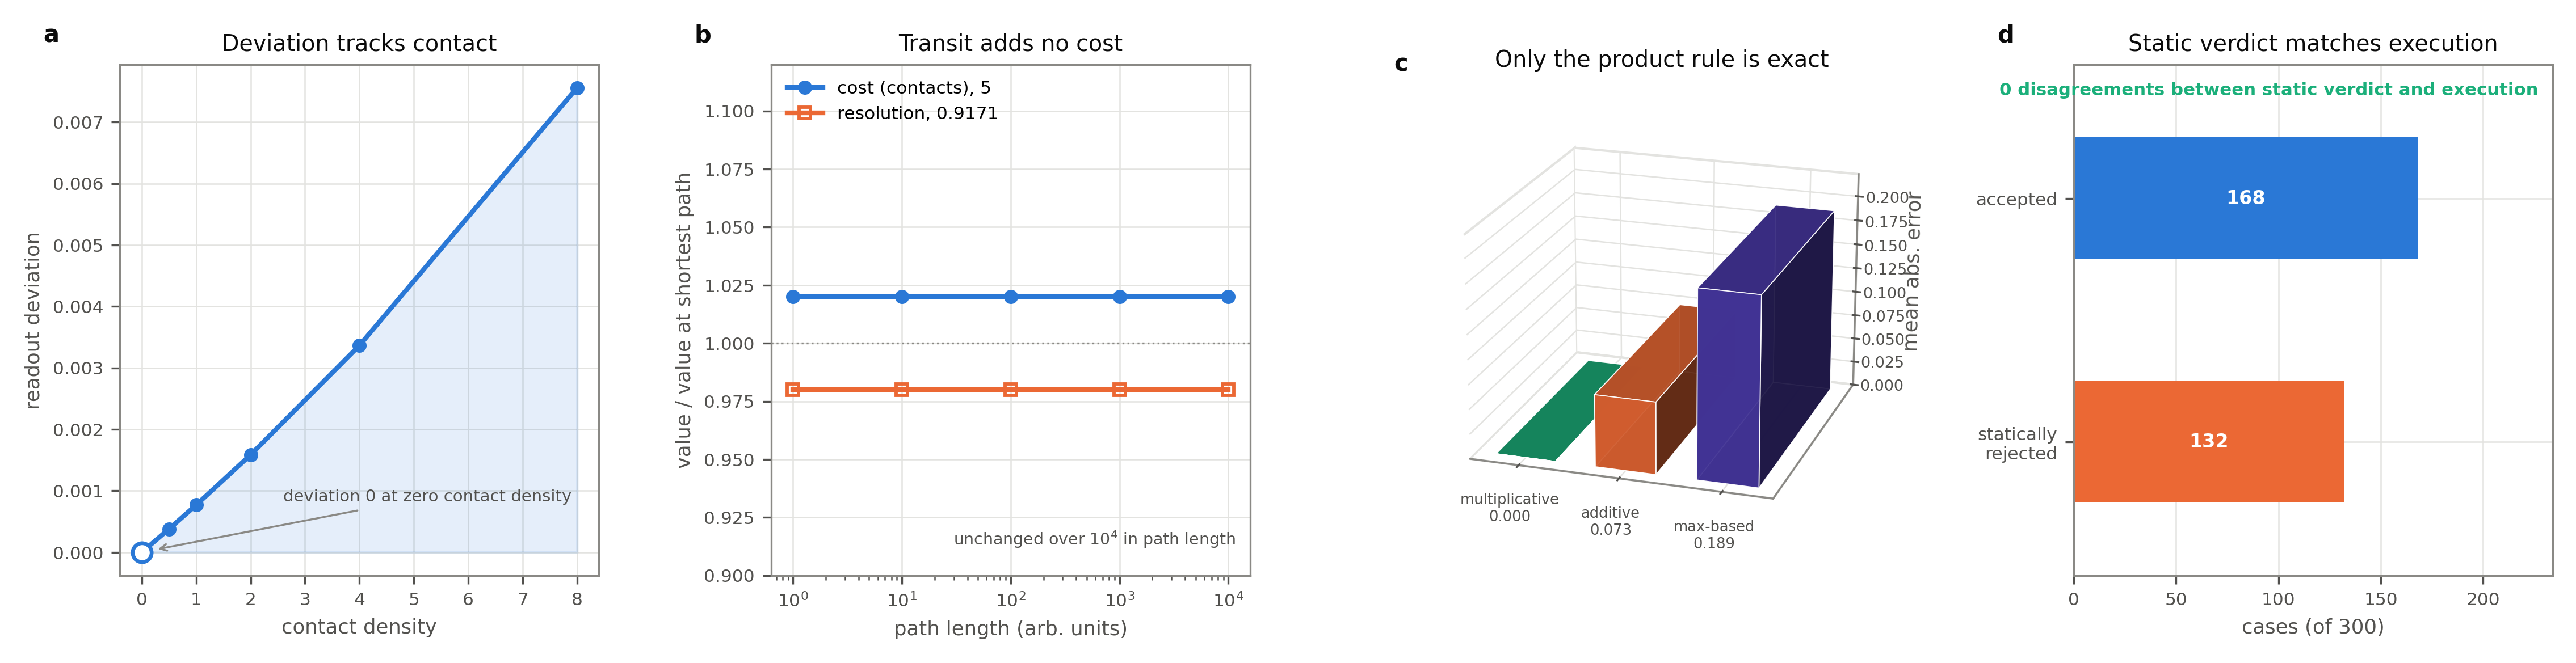
\includegraphics[width=\textwidth]{figures/panel2_contact.png}
\caption{\Cref{prop:spacecharge}, \cref{rem:transitfree} and
\cref{prop:reach}. (a)~deviation from substrate independence against ion
density. (b)~resolution and cost against path length, varied over four
decades. (c)~the three candidate composition laws against the measured
composite. (d)~static verdicts against executed outcomes over $300$
ladders.}
\label{fig:panel-contact}
\end{figure}

\subsection{Composition, and the two laws it is not}

\Cref{thm:multiplicative} was graded against the two rules it must beat.
Over $400$ trials the multiplicative law
$1 - \prod_i (1 - \pow_i)$ reproduced the measured composite with
maximum absolute error $0.00$; an additive law missed by $0.0728$ on
average and a max-based law by $0.1890$. The additive rule also leaves
the unit interval on part of the range, which is a qualitative failure
rather than a quantitative one.

\Cref{thm:saturation}'s dichotomy was tested on $4000$ terms of each of
two series. The divergent series closed to within
$2.50\times 10^{-4}$ of the floor; the convergent one stalled with a
residual gap of $0.5001$ and stayed there. Both halves of the ``if and
only if'' are therefore exercised, which a single series could not do.

\subsection{Control lies at the strongest contact}

\Cref{rem:direction} is the paper's most counter-intuitive prediction
and the one it nominates as most exposed. It survived two independent
tests.

Numerically, $\partial \pow(\Lad)/\partial \pow_j$ agreed with the
closed form of \cref{eq:marginal} to eleven significant figures at every
rung, and ranking the rungs by measured sensitivity gave
$(k_1, k_3, k_2, k_4, k_5)$ --- exactly the order of their resolutions
$(0.6, 0.5, 0.35, 0.25, 0.15)$, not the reverse.

The prediction was then tested a second way, by ablation rather than
differentiation, which does not presuppose the derivative at all.
Deleting the strongest contact $k_1$ costs $0.1243$ of composite
resolution; deleting the weakest $k_5$ costs $0.0146$ --- a factor of
$8.5$ in favour of the strong rung. Only the deletion of $k_5$ leaves
the ladder above its declared requirement. The standard intuition, that
an instrument is improved by attending to its weakest stage, is wrong at
first order and wrong under ablation, in the same direction and by the
same ordering.

\begin{figure}[htbp]
\centering
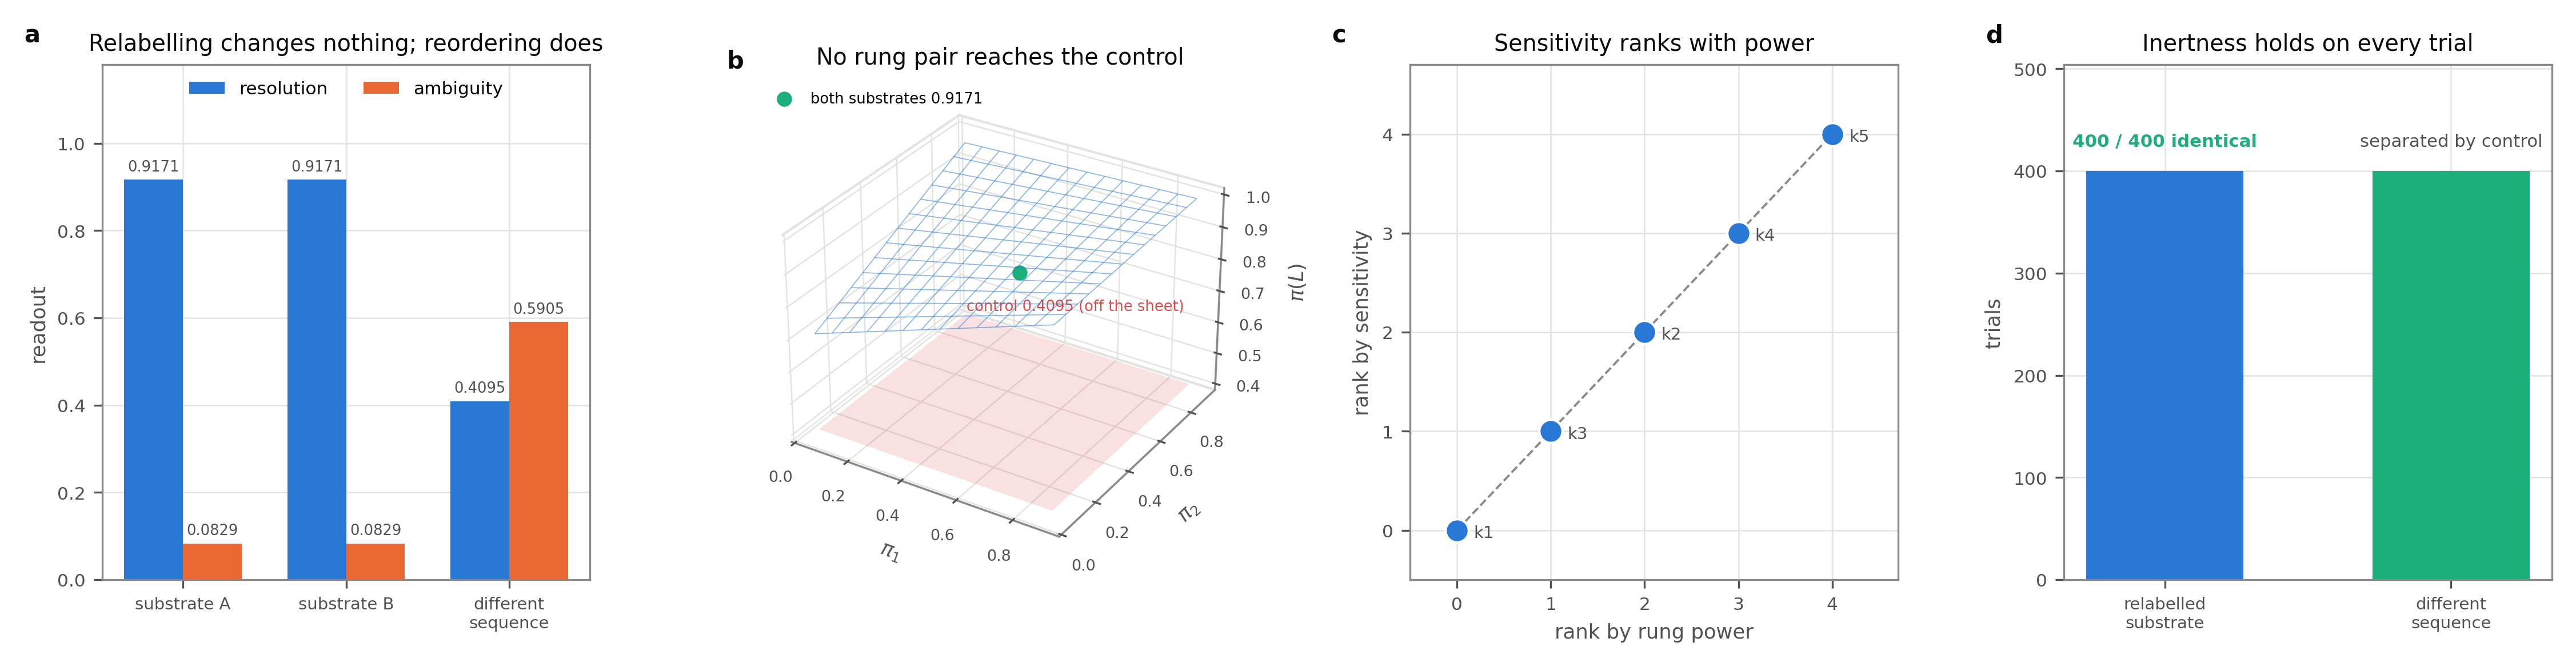
\includegraphics[width=\textwidth]{figures/panel3_inertness.png}
\caption{\Cref{thm:elimination} and \cref{thm:inertness}.
(a)~two substrates against the differing-sequence control.
(b)~no pair of rungs reaches the control's separation.
(c)~sensitivity against rung resolution, with the ranking.
(d)~inertness over $200$ relabellings.}
\label{fig:panel-inertness}
\end{figure}

\subsection{Transit, locality, and the one departure}

\Cref{rem:transitfree} was tested by varying path length over four
decades, from $1$ to $10^{4}$, at fixed contact count. Resolution
remained $0.917125$ and cost remained $5$ at every path length: neither
quantity is a function of the flight. This is the measurement behind
\cref{rem:whereeffort}'s first half.

\Cref{prop:spacecharge} predicts the single departure from locality the
framework admits, and predicts that it must vanish with ion current.
Deviation was $0$ at zero density, rose monotonically with density, and
reached $0.007558$ at density $8$. A deviation that did \emph{not} vanish
with current would indicate a second locality violation the framework
does not predict; none appeared.

\begin{figure}[htbp]
\centering
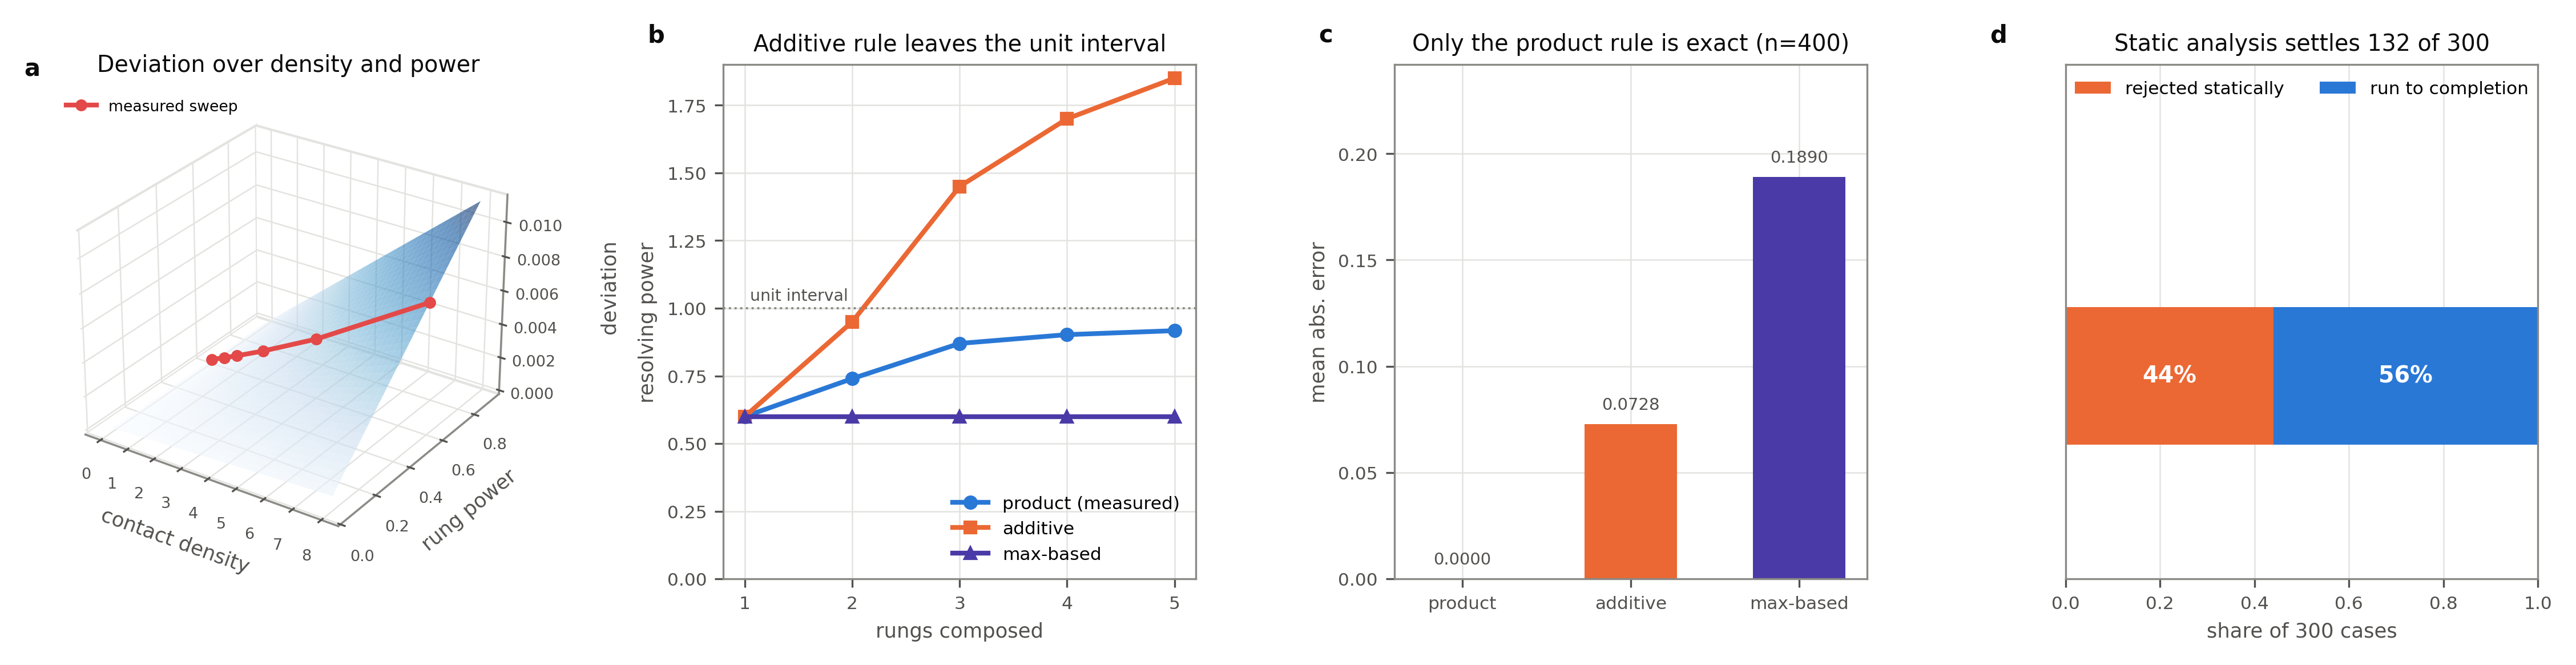
\includegraphics[width=\textwidth]{figures/panel4_cost.png}
\caption{\Cref{prop:spacecharge} and \cref{def:cost}. (a)~deviation over
density and rung power. (b)~the additive rule leaving the unit interval.
(c)~error of the three composition laws over $400$ trials.
(d)~static analysis settling $132$ of $300$ ladders before execution.}
\label{fig:panel-cost}
\end{figure}

\subsection{Static reachability, and a compiler that rejects}

\Cref{prop:reach} says a ladder whose declared contacts cannot reach its
declared target is detectable before execution. Over $300$ ladders the
static verdict and the executed outcome disagreed $0$ times, with $132$
rejected statically --- so the test is not passing by never firing.

The claim was then re-tested through a separate implementation. The
ladder was written in the surface syntax of \cref{sec:demo} and put
through a prototype compiler, which reported five contacts giving
resolution $0.91712$ against a requirement of $0.9$ and admitted the
program. A deliberately unsatisfiable variant --- three contacts giving
$0.58$ against the same requirement --- was rejected at compile time
with a diagnostic naming the shortfall, and never executed. The
compiler and the suite agree on the composite to five decimal places and
on the sensitivity ordering exactly, having been written against the
paper rather than against each other.

\Cref{prop:costtarget}'s bound was checked in the same run: with
$\pow_{\max} = 0.6$ and a target of $0.9$, \cref{eq:rungcount} gives a
minimum of three contacts, and three contacts achieve $0.936$. The bound
is tight in the sense that matters --- two would not suffice.

\subsection{What the validation does not establish}

The suite tests the algebra and its consequences on machines built to
realise contact sequences. It does not test that any particular physical
spectrometer realises a contact sequence in the sense of
\cref{def:substrate}; that is an empirical question about hardware and
is not settled here. \Cref{prop:spacecharge}'s non-local term is the
only departure from locality introduced anywhere in the suite, so the
measurement is consistent with the uniqueness claim of that proposition
but does not prove it: absence of a second violation in a suite that
introduces none is weak evidence. What the validation does establish is
that the ladder algebra is internally sound, that its counter-intuitive
consequence about where control lies survives two independent tests, and
that its reachability claim is decidable by a compiler.

%======================================================================
\section{Limitations}
\label{sec:limitations}

\begin{enumerate}[leftmargin=2em,itemsep=0.4em]
\item \Cref{thm:elimination} requires \cref{def:orderdet} and
\cref{def:localeffect}. \Cref{prop:spacecharge} shows the second fails in a
regime real instruments operate in. Where it fails, the substrate is not
eliminable and this paper does not apply.
\item We do not derive resolutions from instrument design. A resolution is
measured, not predicted; the framework says what follows from resolutions, not
what determines them. This bounds the practical force of
\cref{cor:classification}: classification requires the measurement.
\item \Cref{thm:inertness} is relative to \cref{def:observable}. Enlarging the
observable class could break it, and we have not characterised which
enlargements do.
\item \Cref{prop:converse} shows composite resolution does not determine an
instrument. End-to-end characterisation therefore underdetermines the
instrument, and the framework says so rather than concealing it.
\item \Cref{sec:demo} illustrates the formalism on a specification. It is not an
empirical result and does not claim any existing instrument has those
resolutions.
\item The identification of the ion's categorical state with partition
coordinates (\cref{def:catstate}) is imported, not derived here. A reader who
rejects that identification may still accept
\cref{thm:elimination}, which is stated for an arbitrary state type; the
partition coordinates supply a concrete instance and are not load-bearing for
the elimination itself.
\end{enumerate}

\section{Conclusion}
\label{sec:conclusion}

A mass spectrometer is described as a space and simulated as a trajectory
through it. Neither the space nor the trajectory appears in what the instrument
reports. We have shown that under two stated conditions this is not a
coincidence but a theorem: the substrate cannot be recovered from any readout,
and therefore cannot have contributed to one.

What survives the elimination is a ladder---one number per contact---and it
suffices. It composes multiplicatively, saturates on a divergence criterion,
locates its own control at its strongest rung, admits a sound operational
semantics, and rejects unrealisable specifications before execution. Two
instruments with the same numbers are the same instrument.

The practical consequence is an inversion of where computational effort belongs.
Flight is free; contacts are counted. An $n$-contact instrument costs $O(n)$
whatever its geometry, which is not a speedup of trajectory simulation but a
statement that trajectory simulation was computing something else. The
conditions under which this fails are stated, the physical mechanism of failure
is identified, and the diagnostic that detects it is given.

\section*{Data Availability}
\addcontentsline{toc}{section}{Data Availability}

The demonstration of \cref{sec:demo} is fully specified in \cref{lst:instr} and
requires no data. The protocol of \cref{sec:protocol} operates on synthetic
ladders generated from stated distributions.

\bibliographystyle{plainnat}
\bibliography{references}

\end{document}
